\documentclass{article}
\usepackage{amsmath,amsthm,amssymb,amsfonts}
\usepackage{setspace,enumitem}
\usepackage{graphicx}
\usepackage{hyperref}
\usepackage{natbib}
\usepackage{afterpage}
\usepackage{xcolor}
\usepackage{etoolbox}
\usepackage{booktabs}
\usepackage{pdfpages}
\usepackage{multicol}
\usepackage{geometry}
\usepackage{bbm}
\usepackage{accents}
\hypersetup{
	colorlinks,
	linkcolor={blue!90!black},
	citecolor={red!90!black},
	urlcolor={blue!90!black}
}

\newtheorem{theorem}{Theorem}
\newtheorem{assumption}{Assumption}
\newtheorem{definition}{Definition}
\newtheorem{lemma}{Lemma}
\setlength{\parindent}{0cm}
\geometry{margin = 1in}

\newcommand{\R}{\mathbb{R}}
\newcommand{\ubar}[1]{\underaccent{\bar}{#1}}
\newcommand{\F}{\mathcal{F}}
% \newcommand{\H}{\mathcal{H}}
\newcommand{\xbf}{\mathbf{x}}
\newcommand{\Xbf}{\mathbf{X}}
\newcommand{\Vbf}{\mathbf{V}}
\newcommand{\zbf}{\mathbf{z}}
\newcommand{\Tbf}{\mathbf{T}}
\newcommand{\mubf}{\boldsymbol{\mu}}
\newcommand{\alphabf}{\boldsymbol{\alpha}}
\newcommand{\betabf}{\boldsymbol{\beta}}
\newcommand{\sigmabf}{\boldsymbol{\sigma}}
\newcommand{\onebf}{\mathbbm{1}}
\newcommand{\Covbf}{\text{\textbf{Cov}}}
\newcommand{\Varbf}{\text{\textbf{Var}}}

\newtoggle{extended}
\settoggle{extended}{false}

\title{FIN 971: PS6}

\author{Mitchell Vald\'es-Bobes and Alex von Hafften}

\begin{document}

\maketitle

\subsection*{1. Prove that in this particular problem, all the constraints should be binding}

If $(3)$ holds for both $H$ and $L$, then

\begin{align*}
\begin{cases}
d_H(a) + (1-p_H(a)) \cdot \delta \cdot a'_H(a) + p_H(a) \cdot R \ge \lambda \cdot (Y^H - Y^L) + d_L(a) + (1-p_L(a)) \cdot \delta \cdot a'_L(a) + p_L(a) \cdot R\\
d_L(a) + (1-p_L(a)) \cdot \delta \cdot a'_L(a) + p_L(a) \cdot R \ge \lambda \cdot (Y^L - Y^H) + d_H(a) + (1-p_H(a)) \cdot \delta \cdot a'_H(a) + p_H(a) \cdot R
\end{cases}\\
\implies
\begin{cases}
d_H(a) + (1-p_H(a)) \cdot \delta \cdot a'_H(a) + p_H(a) \cdot R \ge \lambda \cdot (Y^H - Y^L) + d_L(a) + (1-p_L(a)) \cdot \delta \cdot a'_L(a) + p_L(a) \cdot R\\
d_L(a) + (1-p_L(a)) \cdot \delta \cdot a'_L(a) + p_L(a) \cdot R + \lambda \cdot (Y^H - Y^L)\ge  + d_H(a) + (1-p_H(a)) \cdot \delta \cdot a'_H(a) + p_H(a) \cdot R
\end{cases}\\
\implies
d_H(a) + (1-p_H(a)) \cdot \delta \cdot a'_H(a) + p_H(a) \cdot R = \lambda \cdot (Y^H - Y^L) + d_L(a) + (1-p_L(a)) \cdot \delta \cdot a'_L(a) + p_L(a) \cdot R
\end{align*}

Thus, (3) holds with equality.

\bigskip

Clearly, (4) does not hold with equality for $H$ (see policy functions).

\subsection*{2. After solving the problem, graph the value function $b(a)$ and decision rules $d_i(a), p_i(a), a'_i(a)$.}

I ended up coding this problem set in Julia instead of Matlab.  I used the JuMP package for forming the optimization problem and the GLPK package for optimization.  Unfortunately, due to my understanding of JuMP, I was unable to include an interpolated object in the objective function.  Thus, I resorted to using gird search over $a'_H(a)$ and $a'_L(a)$ and then using the constrained optimization methods to get $d_L(a), d_h(a), p_L(a), p_H(a)$.  It wasn't ideal, but I used a number of tricks to speed up the grid search (starting at the previous maximizer and stopping when the value function starts to decrease).  As you can see I find very similar results to slides in class that presumable used fmincon in Matlab.  The waviness of the policy functions come from the grid search.

\bigskip

If the agent reports high cash flow, the principal promises higher future utility (i.e. the $a'_H$ policy function is above the 45 degree line) until a point when the principal start to statically reward the agent (i.e. $d_H$ policy function starts to increase from zero at high enough $a$).  The principal never terminates after a high report.

\bigskip

If the agent reports low cash flow, the principal decreases the promised future utility (i.e. the $a'_L$ policy function is below the 45 degree line). At a certain point, the principal terminates the project after enough low reports (i.e. $p_L$ is positive for low enough $a$).  The principal never rewards the agent after a bad report.

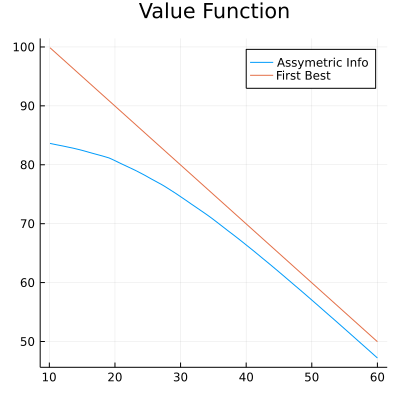
\includegraphics{value_function.png}



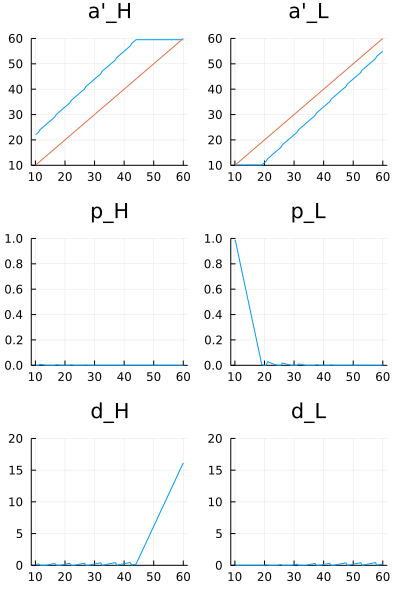
\includegraphics{policy_functions.png}


\end{document}

